\documentclass[a4paper, 11pt]{article}

% Nécessaire
\usepackage[french]{babel}
\usepackage[utf8]{inputenc}
\usepackage[T1]{fontenc}
\usepackage{lmodern}
\usepackage{amsmath, amsthm}
\usepackage{amsfonts,amssymb}

% Marge
\usepackage{geometry}
\geometry{margin={2.2cm ,2cm}}

% Figures, graphiques
\usepackage{graphicx}
\usepackage{epsfig}
\usepackage{caption}

% Surlignage
\usepackage{alltt}

\usepackage{xcolor}
\usepackage{soul}
\usepackage{color}
\usepackage{colortbl}

% Indicatrice
\usepackage{dsfont}

\usepackage{multirow}
\usepackage{eurosym}
\usepackage{extarrows}


% Titre
\title{Modèle conceptuel cécidomyies}
\author{}
\date{}



\begin{document}
\maketitle 

Ce document s'intéresse à la possibilité d'utiliser le nombre de larves qu'il y a eu antérieurement (sur une plage de jours à définir) afin de prédire le nombre de larves au jour $t$.

\section{Régression linéaire simple}

Afin de rester un minimum cohérent avec la littérature, on testera la significativité du nombre de larves qu'il y a eu entre 7 et 17 jours auparavant. Pour ce faire, on effectue pour chacun des trois sous-blocs une régression linéaire simple définit par
$$ L_t = \beta_0 + \sum_{j=7}^{17} \beta_{j} L_{t-j}.$$
Il faut noter que l'on utilisera uniquement les individus vérifiant $t > 17$ jours.

\subsection{Enherbement ras}

Le seuil de significativité sera fixé à $\alpha = 0.05$.
Les résultats de la régression linéaire sont visibles dans la table~\ref{tab:lmer}. Il apparaît que seule l'ordonnée à l'origine est significative. Dès lors, il apparaît compliqué de prédire uniquement le nombre de larves à la date $t$ avec les nombres de larves à des dates antérieures.

\begin{table}[ht]
\centering
\caption{Coefficients trouvés par la régression linéaire simple pour l'enherbement ras, ainsi que leurs erreurs standards associés. Pour un seuil de singnificativité d'$\alpha = 0.05$, seule l'ordonnée à l'origine est significative}
\label{tab:lmer}
\begin{tabular}{rrrrr}
 & Estimate & Std. Error & t value & Pr($>$$|$t$|$) \\ 
  \hline
(Intercept) & 1107.6499 & 184.8822 & 5.99 & 0.0000 \\ 
  `Lt-7' & 0.2387 & 0.3119 & 0.77 & 0.4476 \\ 
  `Lt-8' & -0.1055 & 0.4404 & -0.24 & 0.8117 \\ 
  `Lt-9' & -0.1190 & 0.4329 & -0.27 & 0.7845 \\ 
  `Lt-10' & -0.1849 & 0.4171 & -0.44 & 0.6593 \\ 
  `Lt-11' & -0.0115 & 0.4128 & -0.03 & 0.9779 \\ 
  `Lt-12' & -0.0087 & 0.4095 & -0.02 & 0.9831 \\ 
  `Lt-13' & -0.0624 & 0.4179 & -0.15 & 0.8819 \\ 
  `Lt-14' & 0.3418 & 0.4333 & 0.79 & 0.4339 \\ 
  `Lt-15' & -0.0895 & 0.4401 & -0.20 & 0.8396 \\ 
  `Lt-16' & 0.0927 & 0.5126 & 0.18 & 0.8572 \\ 
  `Lt-17' & -0.4645 & 0.4066 & -1.14 & 0.2587 
\end{tabular}
\end{table}

La figure~\ref{fig:lmer1} montre ainsi la tendance du modèle à renvoyer pour tout les individus une valeur dans une plage de valeurs assez restreinte, ne reflétant pas la variabilité des observations. Ce faisant, le modèle proposé renvoie ainsi une valeur moyenne ne tenant finalement assez peu compte de la valeur au jour $t$. La figure~\ref{fig:lmer2} confirme cette tendance en montrant la piètre qualité de la prédiction.

\begin{figure}[ht]
 \centering
 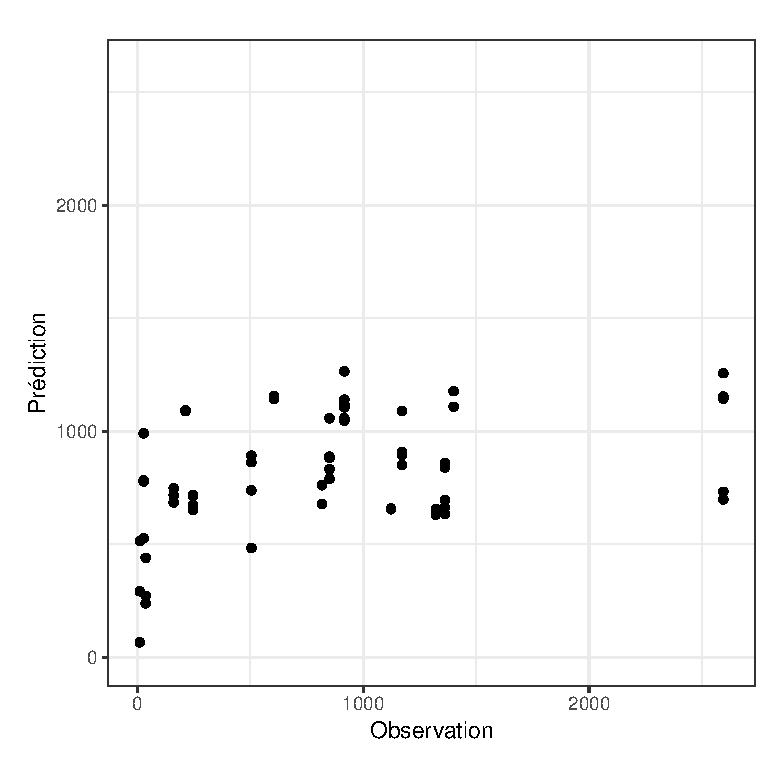
\epsfig{file = plots/pred_obs_ER.eps, scale = 0.65}
 \caption{Comparaison entre les valeurs observées et les valeurs prédites pour l'enherbement ras. Une bonne prédiction montrerait les points proches de la doite $y=x$. Ce n'est pas le cas ici.}
 \label{fig:lmer1}
\end{figure}

\begin{figure}[ht]
 \centering
 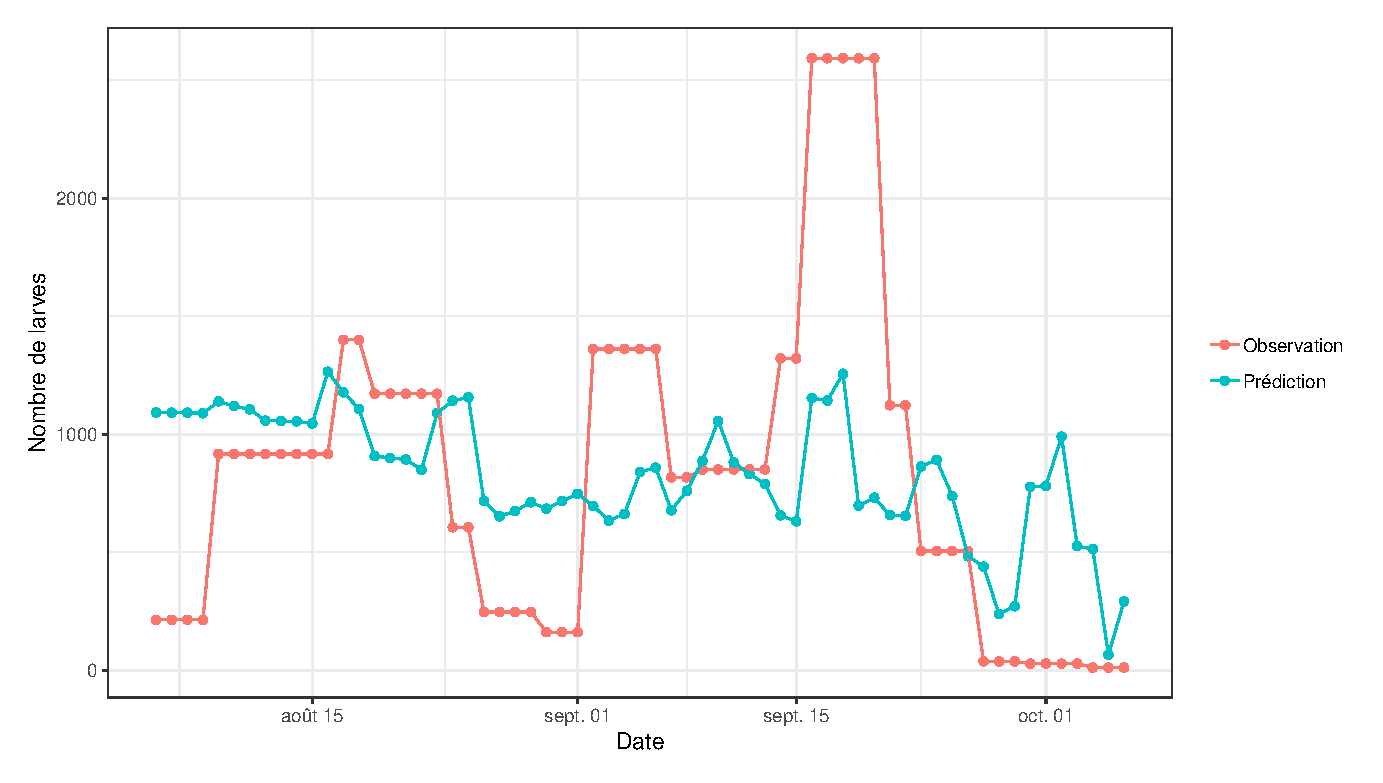
\epsfig{file = plots/pred_ER2.eps, scale = 0.65}
 \caption{Comparaison des nombres larves observées et des larves prédites à chaque date pour l'enherbement ras. La prédiction --- plutôt mauvaise --- renvoie une valeur assez proche tous les jours, ne captant  pas la dynamique du phénomène observé.}
 \label{fig:lmer2}
\end{figure}

\subsection{Paillage synthétique}

On réitère les calculs pour le paillage synthétique. Les résultats sont visibles dans la table~\ref{tab:lmps}, et comme pour l'enherbement ras seul l'ordonnée à l'origine est significative. Ainsi il n'est pas étonnant de trouver des résultats similaires concernant la prédiction comme l'illustre les figures~\ref{fig:lmps1} et \ref{fig:lmps2} : une prédiction mauvaise qui donne une valeur moyenne tout du long, manquant de réalisme.

\begin{table}[ht]
\centering
\caption{Coefficients trouvés par la régression linéaire simple pour le paillage synthétique, ainsi que leurs erreurs standards associés. Pour un seuil de singnificativité d'$\alpha = 0.05$, seule l'ordonnée à l'origine est significative}
\label{tab:lmps}
\begin{tabular}{rrrrr}
  
 & Estimate & Std. Error & t value & Pr($>$$|$t$|$) \\ 
  \hline
(Intercept) & 296.6741 & 78.6914 & 3.77 & 0.0004 \\ 
  `Lt-7' & 0.4112 & 0.3590 & 1.15 & 0.2575 \\ 
  `Lt-8' & 0.0161 & 0.5157 & 0.03 & 0.9753 \\ 
  `Lt-9' & -0.1417 & 0.5647 & -0.25 & 0.8029 \\ 
  `Lt-10' & -0.1033 & 0.5208 & -0.20 & 0.8435 \\ 
  `Lt-11' & 0.0148 & 0.4569 & 0.03 & 0.9743 \\ 
  `Lt-12' & 0.1155 & 0.4571 & 0.25 & 0.8015 \\ 
  `Lt-13' & -0.1878 & 0.4617 & -0.41 & 0.6858 \\ 
  `Lt-14' & 0.0936 & 0.5074 & 0.18 & 0.8544 \\ 
  `Lt-15' & 0.0908 & 0.5323 & 0.17 & 0.8652 \\ 
  `Lt-16' & -0.0222 & 0.7469 & -0.03 & 0.9764 \\ 
  `Lt-17' & -0.2156 & 0.6257 & -0.34 & 0.7319 
\end{tabular}
\end{table}

\begin{figure}[ht]
 \centering
 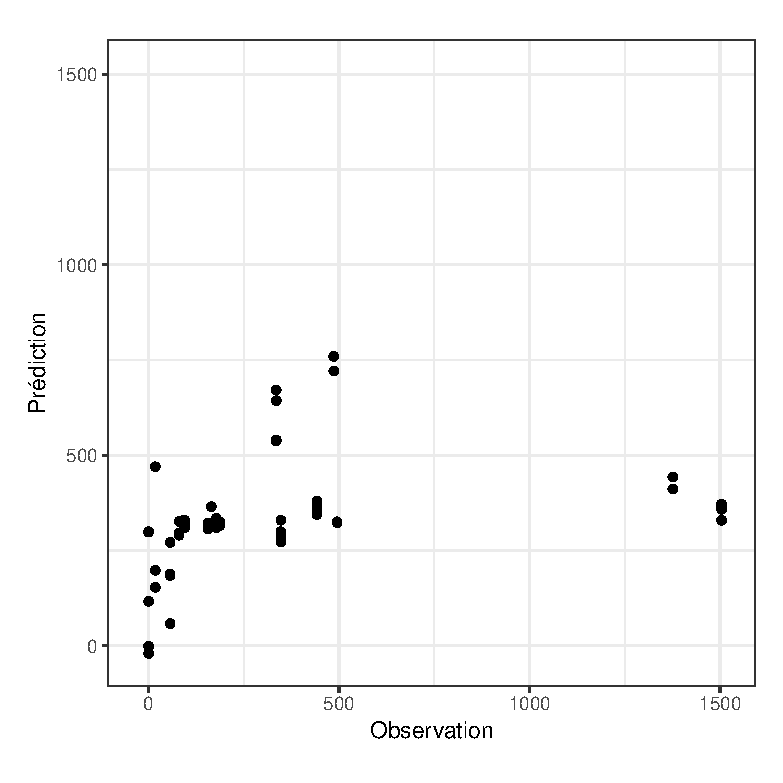
\epsfig{file = plots/pred_obs_PS.eps, scale = 0.65}
 \caption{Comparaison entre les valeurs observées et les valeurs prédites pour le paillage synthétique. Une bonne prédiction montrerait les points proches de la doite $y=x$. Ce n'est pas le cas ici.}
 \label{fig:lmps1}
\end{figure}

\begin{figure}[ht]
 \centering
 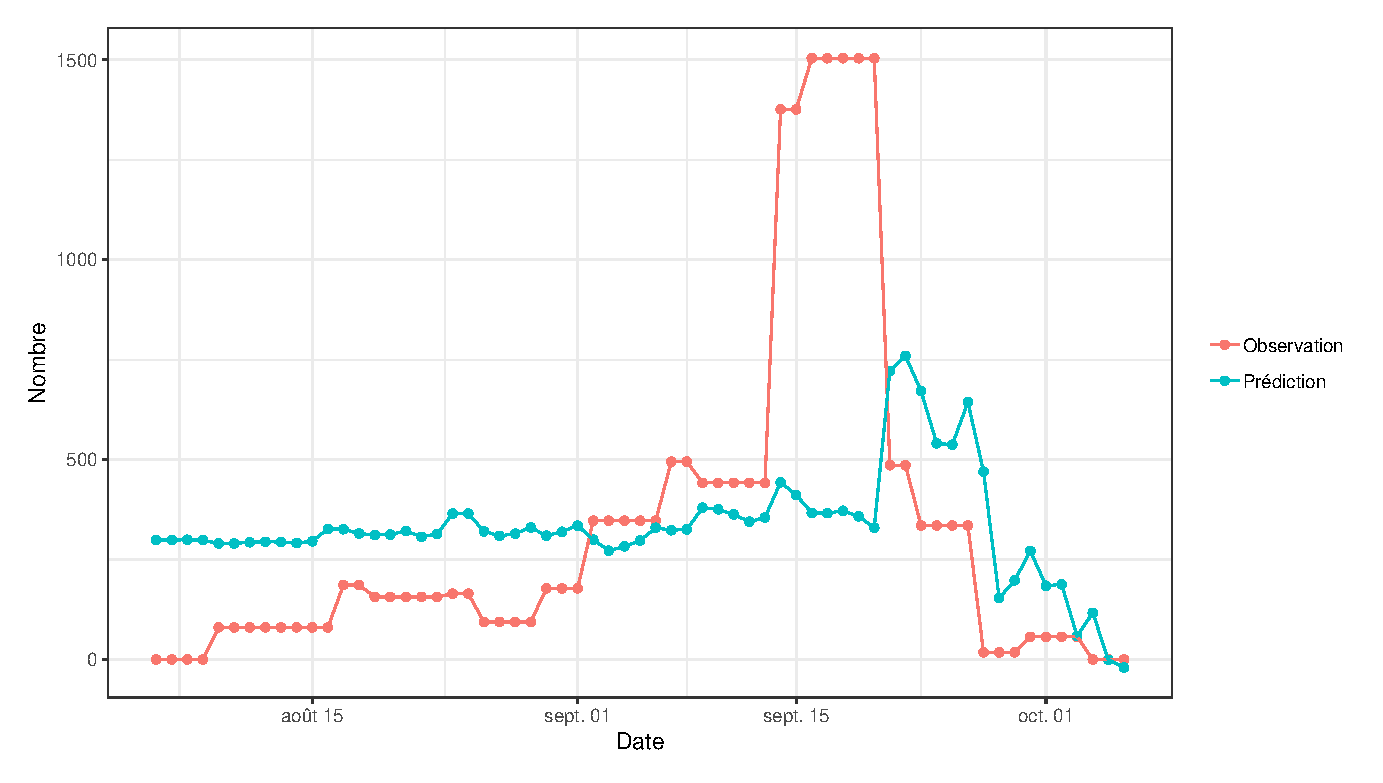
\epsfig{file = plots/pred_PS2.eps, scale = 0.65}
 \caption{Comparaison des nombres larves observées et des larves prédites à chaque date pour le paillage synthétique. La prédiction --- plutôt mauvaise --- renvoie une valeur assez proche tous les jours, ne captant  pas la dynamique du phénomène observé.}
 \label{fig:lmps2}
\end{figure}

\subsection{Enherbement haut}

Encore une fois, seule l'ordonnée à l'origine est significative (voir table~\ref{tab:lmeh}). Cependant la figure~\ref{fig:lmeh1} montre des prédictions plus variables, qui si elles ne sont pas parfaites (particulièrement vrai pour les valeurs observées très grande ou très petites) demeurent bien supérieures aux deux autres sous-blocs. Cela se vérifie sur la figure~\ref{fig:lmeh2} où l'on peut voir que la dynamique est plus ou moins captée (moins que plus, il est vrai).

\begin{table}[ht]
\centering
\caption{Coefficients trouvés par la régression linéaire simple pour l'enherbement haut, ainsi que leurs erreurs standards associés. Pour un seuil de singnificativité d'$\alpha = 0.05$, seule l'ordonnée à l'origine est significative}
\label{tab:lmeh}
\begin{tabular}{rrrrr}
 & Estimate & Std. Error & t value & Pr($>$$|$t$|$) \\ 
  \hline
(Intercept) & 525.1541 & 159.7604 & 3.29 & 0.0018 \\ 
  `Lt-7' & 0.5592 & 0.3297 & 1.70 & 0.0960 \\ 
  `Lt-8' & -0.1018 & 0.4635 & -0.22 & 0.8270 \\ 
  `Lt-9' & 0.2186 & 0.4608 & 0.47 & 0.6372 \\ 
  `Lt-10' & 0.0512 & 0.4636 & 0.11 & 0.9125 \\ 
  `Lt-11' & -0.3174 & 0.4741 & -0.67 & 0.5062 \\ 
  `Lt-12' & 0.2680 & 0.4781 & 0.56 & 0.5776 \\ 
  `Lt-13' & -0.2279 & 0.4834 & -0.47 & 0.6392 \\ 
  `Lt-14' & 0.3811 & 0.5218 & 0.73 & 0.4685 \\ 
  `Lt-15' & -0.1342 & 0.5405 & -0.25 & 0.8048 \\ 
  `Lt-16' & -0.1415 & 0.5491 & -0.26 & 0.7977 \\ 
  `Lt-17' & -0.2839 & 0.4105 & -0.69 & 0.4923 \\ 
\end{tabular}
\end{table}

\begin{figure}[ht]
 \centering
 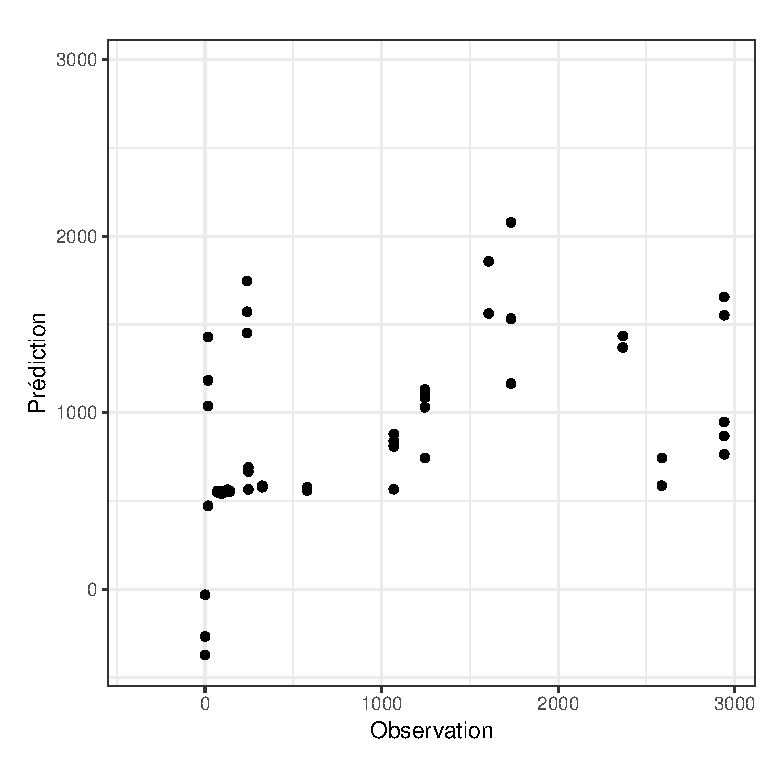
\epsfig{file = plots/pred_obs_EH.eps, scale = 0.65}
 \caption{Comparaison entre les valeurs observées et les valeurs prédites pour l'enherbement haut. Une bonne prédiction montrerait les points proches de la doite $y=x$. La prédiction n'est pas géniale ici.}
 \label{fig:lmeh1}
\end{figure}

\begin{figure}[ht]
 \centering
 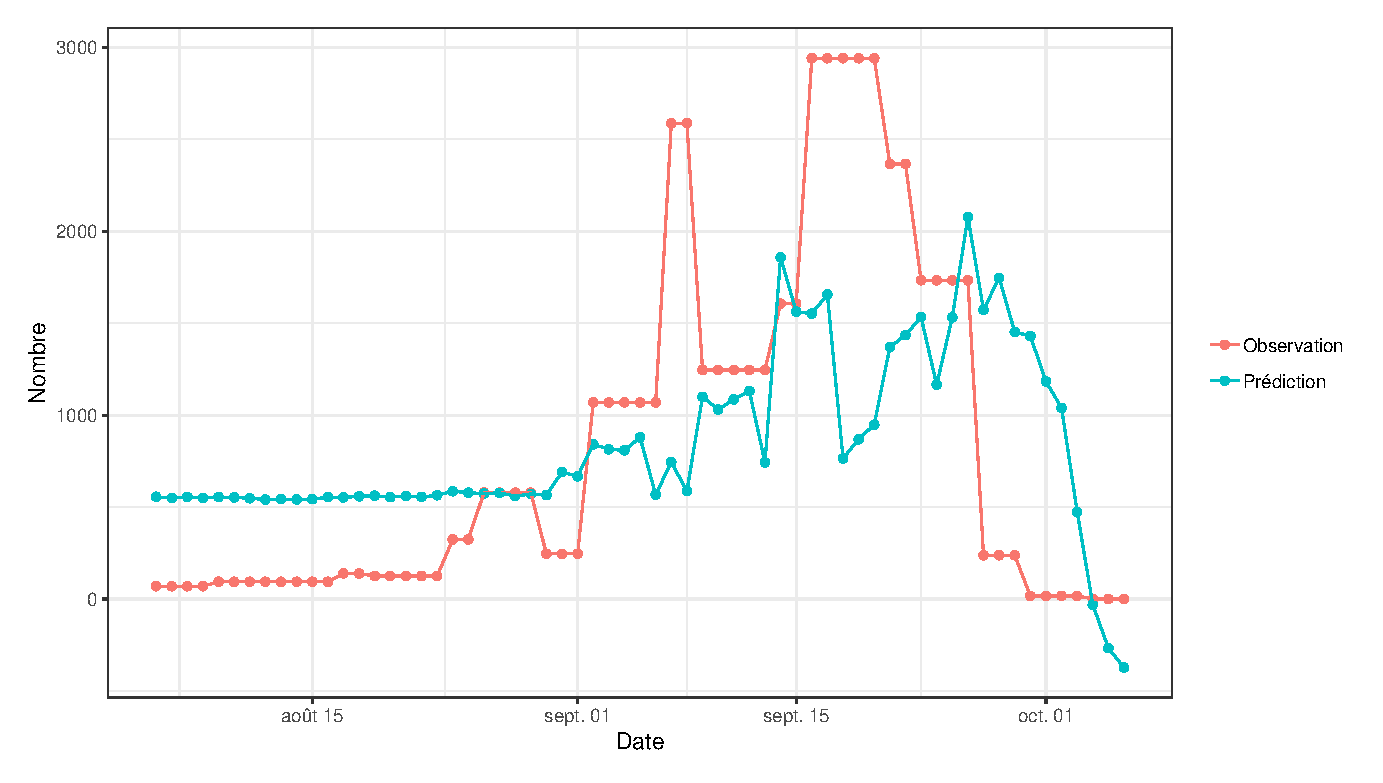
\epsfig{file = plots/pred_EH2.eps, scale = 0.65}
 \caption{Comparaison des nombres larves observées et des larves prédites à chaque date pour l'enherbement haut. La prédiction arrive  à capter très grossièrement le phénomène observé. }
 \label{fig:lmeh2}
\end{figure}

\clearpage
\subsection{Conclusion}

Les résultats présentés ici indiquent clairement que le nombre de larves au jour $t$ ne peut être modélisé par une combinaison linéaire des nombres de larves qu'il y a eu quelques jours plus tôt.

D'autres méthodes ont étés testés, notamment un GLM Poisson et un GLM gaussien. Bien qu'il en ressortait que certaines variables étaient significatives, les prédictions étaient tout aussi mauvaises et similaires à la régression linéaire simple.

Enfin un modèle linéaire mixte a été réalisé sur l'ensemble de la parcelle avec la modalité de couverture de sol comme effet fixe. Il en ressort qu'il y avait une différence significative entre les trois modalités de couverture du sol, ce qui est encourageant dans la mesure que cela implique que ce facteur est utile pour expliquer les différences entre les trois sous-blocs.

\section{Corrélations}

On s'intéresse maintenant à l'autocorrélation des larves et la corrélation entre les larves et les inflorescences. Le coefficient de corrélation de Spearman sera utilisé.

\subsection{Autocorrélation}

On calcule l'autocorrélation des larves avec un \emph{lag} allant de 7 à 17 jours. Les résultats sont les suivants:

\begin{center}
\begin{tabular}{rrrr}
 & Enherbement ras & Paillage synthétique & Enherbement haut \\
$\rho\left( L_t, L_{t-7} \right)    $ &  0.292 & 0.613 & 0.574\\
$\rho\left( L_t, L_{t-8} \right)    $&  0.199 &  0.549 & 0.526 \\
$\rho\left( L_t, L_{t-9} \right)    $&  0.080&   0.462 & 0.475\\
$\rho\left( L_t, L_{t-10} \right)    $&  0.013&  0.379 & 0.408 \\
$\rho\left( L_t, L_{t-11} \right)    $& -0.012 & 0.338 & 0.381 \\
$\rho\left( L_t, L_{t-12} \right)    $& -0.032 & 0.299 & 0.364     \\
$\rho\left( L_t, L_{t-13} \right)    $& -0.083 & 0.260 & 0.342    \\
$\rho\left( L_t, L_{t-14} \right)    $& -0.110 & 0.220 & 0.326         \\
$\rho\left( L_t, L_{t-15} \right)    $& -0.153 & 0.186 & 0.307          \\
$\rho\left( L_t, L_{t-16} \right)    $& -0.182 & 0.156 & 0.285           \\
$\rho\left( L_t, L_{t-17} \right)    $& -0.239 & 0.127 & 0.271             
\end{tabular}
\end{center}

L'autocorrélation est assez faible, en particulier pour l'enherbement ras. De plus cette autocorrélation n'a pas l'air de prendre en compte le cycle de développement des cécidomyies, elle est décroissante avec le temps alors que l'on s'attendrait à pic aux alentours de 12 -- 14 jours (correspondant à un cycle complet) --- exception faite pour l'enherbement ras, avec des corrélations qui remontent légèrement à la fin. 

\subsection{Corrélation entre les larves et les inflorescences}

On s'intéresse maintenant à la corrélation entre les larves et les inflorescences. On fait toujours varier le \emph{lag} entre 7 et 17 jours. Les résultats sont visibles ci-dessous :

\begin{center}
\begin{tabular}{rrrr}
 & Enherbement ras & Paillage synthétique & Enherbement haut \\
$\rho\left( L_t, I_{t-7} \right)    $ & 0.522& 0.351& 0.580 \\
$\rho\left( L_t, I_{t-8} \right)    $ & 0.422& 0.298& 0.556  \\
$\rho\left( L_t, I_{t-9} \right)    $ & 0.325& 0.258& 0.529   \\
$\rho\left( L_t, I_{t-10} \right)    $& 0.244& 0.243& 0.494    \\
$\rho\left( L_t, I_{t-11} \right)    $& 0.185& 0.234& 0.466     \\
$\rho\left( L_t, I_{t-12} \right)    $& 0.123& 0.217& 0.442      \\
$\rho\left( L_t, I_{t-13} \right)    $& 0.064& 0.181& 0.401       \\
$\rho\left( L_t, I_{t-14} \right)    $& 0.015& 0.127& 0.357      \\
$\rho\left( L_t, I_{t-15} \right)    $& -0.021&  0.062&  0.326    \\
$\rho\left( L_t, I_{t-16} \right)    $& -0.020& -0.001&  0.294  \\
$\rho\left( L_t, I_{t-17} \right)    $&  0.007& -0.063& 0.275
\end{tabular}
\end{center}


Un phénomène quelque peu semblable à l'autocorrélation des larves est présent. Une décroissance avec le temps d'une corrélation qui n'était pas bien forte au début. Cela reste néamoins plus intéprétable dans la mesure où la corrélation la plus importante coïncide avec la durée de larvation. Il convient cependant de rester prudent dans la mesure où l'on n'observe pas une franche diminution après la durée de larvation, ce qui semble plus indiquer que cela reste un phénomène lié au temps et indépendant du cycle de développement des cécidomyies.


\subsection{Conclusion}

Les corrélations calculées précedemment semblent en accord avec les résultats de la première partie. À savoir que les larves et les inflorescences ne peuvent (du moins linéairement) prédire le nombre de larves à venir. Cela a au moins le mérite de comforter l'approche choisie, à savoir un modèle décrivant les phénomènes observés.

\section{Modèle conceptuel}

On s'intéresse au modèle conceptuel
$$L_t = \alpha(t) R \left( \mu L_{t-12} + E(t-7) \right),$$
où $R$ représente le coefficient de reproduction des femelles, $\mu$ la probabilité de survie des œufs, $E(t-7)$ les individus exogènes arrivant 7 jours avant, $L_{t-12}$ le nombre de larves présentes un cycle auparavant et $\alpha(t)$ un coefficient journalier représentant l'ensemble des conditions environnementales.

\end{document}

